\begin{figure}[h!]
	\centering
	
	
	\tikzset{every picture/.style={line width=0.75pt}} %set default line width to 0.75pt        
	
	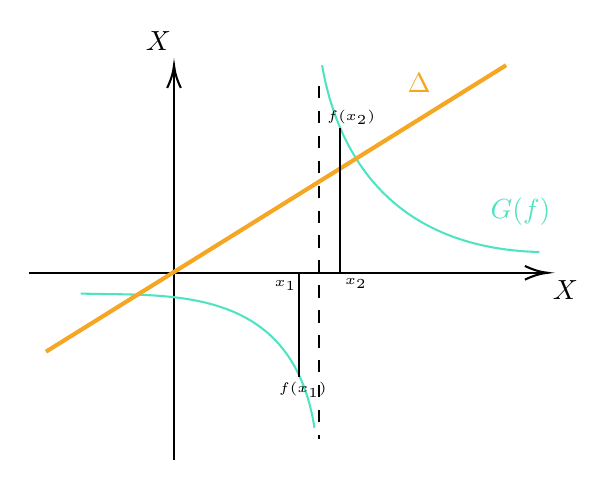
\begin{tikzpicture}[x=0.75pt,y=0.75pt,yscale=-1,xscale=1]
		%uncomment if require: \path (0,300); %set diagram left start at 0, and has height of 300
		
		%Straight Lines [id:da19790917179960688] 
		\draw    (180,140) -- (428,140) ;
		\draw [shift={(430,140)}, rotate = 180] [color={rgb, 255:red, 0; green, 0; blue, 0 }  ][line width=0.75]    (10.93,-3.29) .. controls (6.95,-1.4) and (3.31,-0.3) .. (0,0) .. controls (3.31,0.3) and (6.95,1.4) .. (10.93,3.29)   ;
		%Straight Lines [id:da6463205087944646] 
		\draw    (250,230) -- (250,42) ;
		\draw [shift={(250,40)}, rotate = 90] [color={rgb, 255:red, 0; green, 0; blue, 0 }  ][line width=0.75]    (10.93,-3.29) .. controls (6.95,-1.4) and (3.31,-0.3) .. (0,0) .. controls (3.31,0.3) and (6.95,1.4) .. (10.93,3.29)   ;
		%Straight Lines [id:da7329652606719634] 
		\draw  [dash pattern={on 4.5pt off 4.5pt}]  (320,50) -- (320,220) ;
		%Curve Lines [id:da792914158474481] 
		\draw [color={rgb, 255:red, 80; green, 227; blue, 194 }  ,draw opacity=1 ]   (321.33,40) .. controls (328.33,80.33) and (352.67,128) .. (426,130) ;
		%Curve Lines [id:da5357944547931757] 
		\draw [color={rgb, 255:red, 80; green, 227; blue, 194 }  ,draw opacity=1 ]   (317.67,214.67) .. controls (306.67,144.67) and (246.67,151.33) .. (205,150) ;
		%Straight Lines [id:da25095847185427966] 
		\draw [color={rgb, 255:red, 245; green, 166; blue, 35 }  ,draw opacity=1 ][line width=1.5]    (188.33,178) -- (410,40) ;
		%Straight Lines [id:da14232861437954414] 
		\draw    (310,140) -- (310,190) ;
		%Straight Lines [id:da822434531716816] 
		\draw    (330,70) -- (330,140) ;
		
		% Text Node
		\draw (431,142.4) node [anchor=north west][inner sep=0.75pt]    {$X$};
		% Text Node
		\draw (235,22.4) node [anchor=north west][inner sep=0.75pt]    {$X$};
		% Text Node
		\draw (401,102.4) node [anchor=north west][inner sep=0.75pt]  [color={rgb, 255:red, 80; green, 227; blue, 194 }  ,opacity=1 ]  {$G( f)$};
		% Text Node
		\draw (361,42.4) node [anchor=north west][inner sep=0.75pt]  [color={rgb, 255:red, 245; green, 166; blue, 35 }  ,opacity=1 ]  {$\Delta $};
		% Text Node
		\draw (297,142.4) node [anchor=north west][inner sep=0.75pt]  [font=\tiny]  {$x_{1}$};
		% Text Node
		\draw (331,141.4) node [anchor=north west][inner sep=0.75pt]  [font=\tiny]  {$x_{2}$};
		% Text Node
		\draw (322.33,60.07) node [anchor=north west][inner sep=0.75pt]  [font=\tiny]  {$f( x_{2})$};
		% Text Node
		\draw (299,191.4) node [anchor=north west][inner sep=0.75pt]  [font=\tiny]  {$f( x_{1})$};
		
		
	\end{tikzpicture}
\end{figure}